\documentclass{article}
\usepackage[margin=0.25in]{geometry}
\usepackage{pgfplots}
\usepackage{tikz}
\begin{document}
  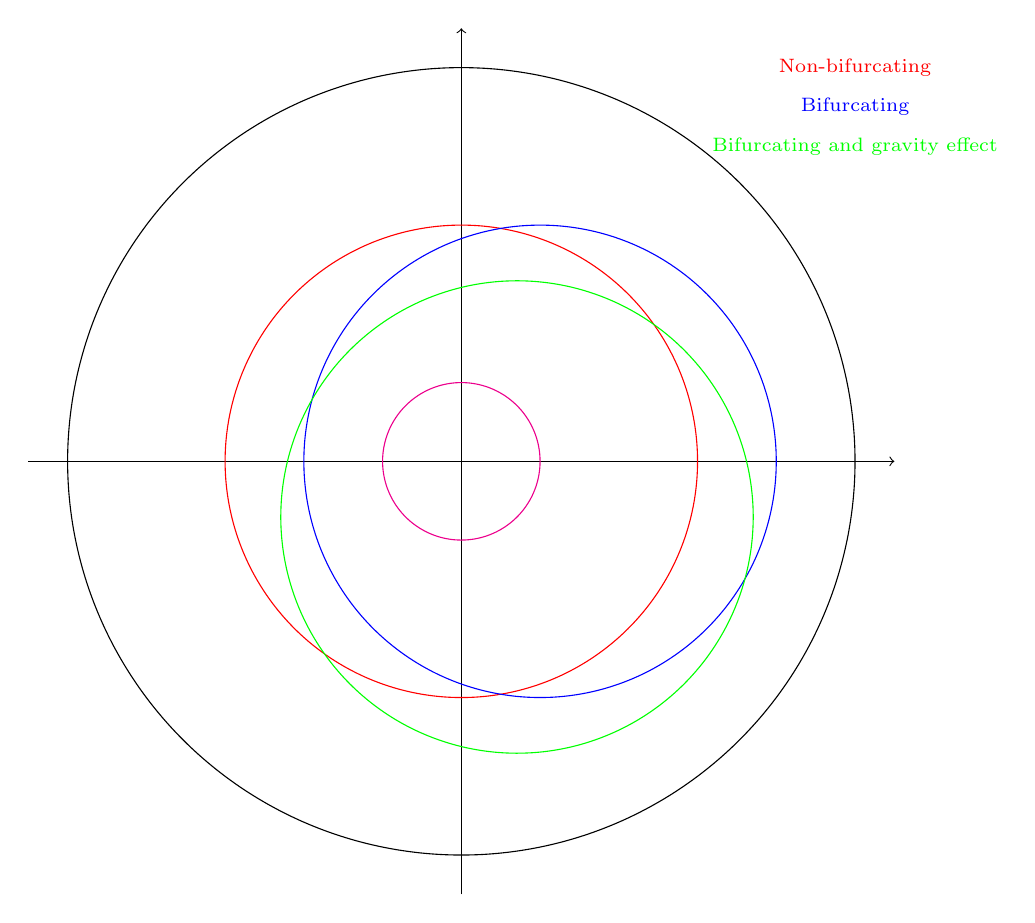
\begin{tikzpicture}[scale=0.1]
  \draw[->] (-55,0) -- (55,0);
  \draw[->] (0,-55) -- (0,55);
  \draw node [red] at (50,50) {\scriptsize{Non-bifurcating}};
  \draw node [blue] at (50,45) {\scriptsize{Bifurcating}};
  \draw node [green] at (50,40) {\scriptsize{Bifurcating and gravity effect}};
  \draw[color=black,domain=0:2*pi,samples=200,smooth] plot (xy polar
  cs:angle=\x r,radius= {50});    %r = angle en radian
  \draw[color=red,domain=0:2*pi,samples=200,smooth] plot (xy polar
  cs:angle=\x r,radius= {30});    %r = angle en radian
  \draw[color=blue,domain=0:2*pi,samples=200,smooth] plot (xy polar
  cs:angle=\x r,radius= {10*cos(\x r) + (30^2-10^2*sin(\x r)^2)^0.5});
  \draw[color=green,domain=0:2*pi,samples=200,smooth] plot (xy polar
  cs:angle=\x r,radius= {10*cos(\x r + 45) + (30^2-10^2*sin(\x r + 45)^2)^0.5});
  \draw[color=magenta,domain=0:2*pi,samples=200,smooth] plot (xy polar
  cs:angle=\x r,radius= {10});
  \end{tikzpicture}
\end{document}